\section{Biological Introduction}
\emph{Chronological ID:} \texttt{2024-02-29:01}

\emph{Structural ID:} \texttt{3}

After first forming on the *Earth via the process of abiogenesis as stated in section \texttt{2.10}, the primordial lifeforms reproduced and evolved, subject to the principles of Darwinian evolution, and occasionally affected by mass extinctions that eliminated entire clades.

\begin{figure}[h]
  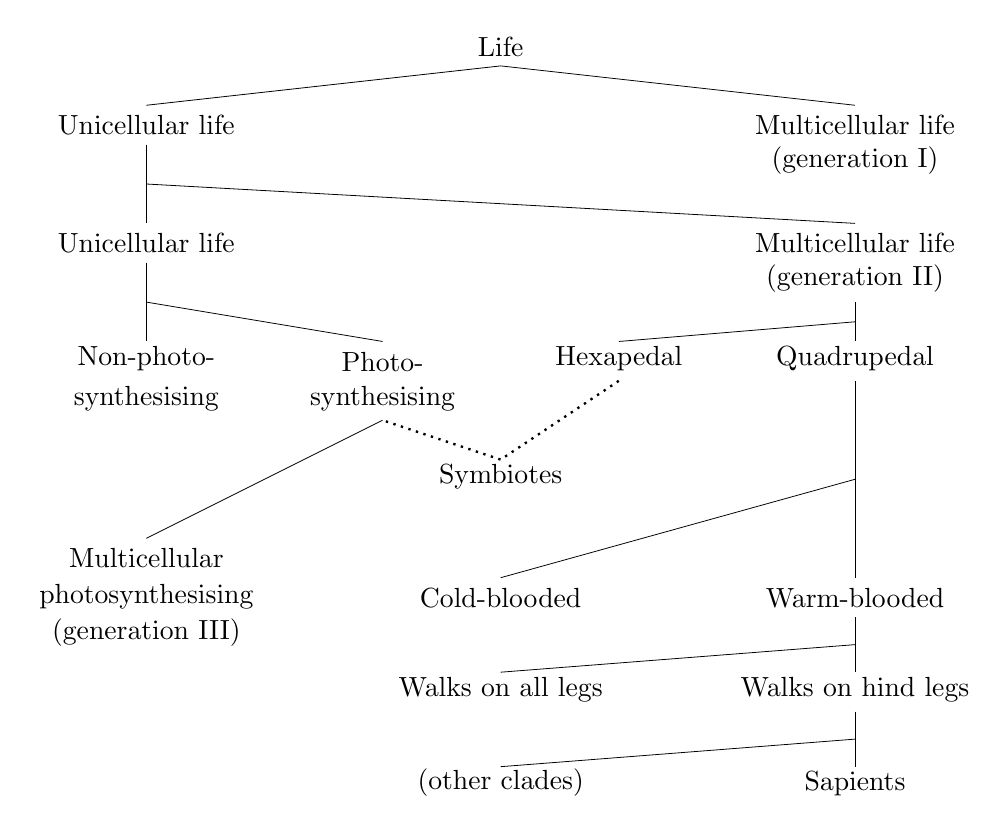
\begin{tikzpicture}
    \draw[white] (0,0);
    \node[anchor=south] (ll) at (6, 0){Life};
    \draw[black,line width=0.01cm] (10.5,-0.5) -- (6,0) -- (1.5, -0.5);
    \node[anchor=south] (lul) at (1.5, -1){Unicellular life};
    \node[anchor=south] (lmli) at (10.5, -1){Multicellular life};
    \node[anchor=south] (lmli2) at (10.5, -1.5){(generation I) \Cross};
    \draw[black,line width=0.01cm] (1.5,-1) -- (1.5, -2);
    \draw[black,line width=0.01cm] (1.5,-1.5) -- (10.5, -2);
    \node[anchor=south] (lul2) at (1.5, -2.5){Unicellular life};
    \node[anchor=south] (lmlii) at (10.5, -2.5){Multicellular life};
    \node[anchor=south] (lmlii2) at (10.5, -3){(generation II)};
    \draw[black,line width=0.01cm] (1.5,-2.5) -- (1.5, -3.5);
    \draw[black,line width=0.01cm] (1.5,-3) -- (4.5, -3.5);
    \draw[black,line width=0.01cm] (10.5,-3) -- (10.5, -3.5);
    \draw[black,line width=0.01cm] (10.5,-3.25) -- (7.5, -3.5);
    \node[anchor=south] (lnp) at (1.5, -4){Non-photo-};
    \node[anchor=south] (lnp2) at (1.5, -4.5){synthesising};
    \node[anchor=south] (lp) at (4.5, -4){Photo-};
    \node[anchor=south] (lp2) at (4.5, -4.5){synthesising};
    \node[anchor=south] (lhp) at (7.5, -4){Hexapedal};
    \node[anchor=south] (lqp) at (10.5, -4){Quadrupedal};
    \draw[black,line width=0.03cm,dotted] (7.5,-4) -- (6, -5) -- (4.5,-4.5);
    \draw[black,line width=0.01cm] (4.5,-4.5) -- (1.5, -6);
    \draw[black,line width=0.01cm] (10.5,-4) -- (10.5, -6.5);
    \draw[black,line width=0.01cm] (10.5,-5.25) -- (6, -6.5);
    \node[anchor=south] (lsym) at (6, -5.5){Symbiotes};
    \node[anchor=south] (lpiii) at (1.5, -6.5){Multicellular};
    \node[anchor=south] (lpiii2) at (1.5, -7.02){photosynthesising};
    \node[anchor=south] (lpiii3) at (1.5, -7.5){(generation III)};
    \node[anchor=south] (lcb) at (6, -7){Cold-blooded};
    \node[anchor=south] (lwb) at (10.5, -7){Warm-blooded};
    \draw[black,line width=0.01cm] (10.5,-7) -- (10.5, -7.7);
    \draw[black,line width=0.01cm] (10.5,-7.35) -- (6, -7.7);
    \node[anchor=south] (lal) at (6, -8.2){Walks on all legs};
    \node[anchor=south] (lhl) at (10.5, -8.2){Walks on hind legs};
    \draw[black,line width=0.01cm] (10.5,-8.2) -- (10.5, -8.9);
    \draw[black,line width=0.01cm] (10.5,-8.55) -- (6, -8.9);
    \node[anchor=south] (loc) at (6, -9.4){(other clades)};
    \node[anchor=south] (lsap) at (10.5, -9.4){Sapients};
  \end{tikzpicture}
  \caption{A rough tree of life, naming the most prominent forms of life on the *Earth.}
\end{figure}
\newpage
